\documentclass[8pt,aspectratio=169]{beamer}
\usetheme{Madrid}
\usepackage{graphicx}
\usepackage{booktabs}
\usepackage{adjustbox}
\usepackage{multicol}
\usepackage{amsmath}
\usepackage{amssymb}
\usepackage{listings}
\usepackage{xcolor}

% Color definitions
\definecolor{mlblue}{RGB}{0,102,204}
\definecolor{mlpurple}{RGB}{51,51,178}
\definecolor{mllavender}{RGB}{173,173,224}
\definecolor{mllavender2}{RGB}{193,193,232}
\definecolor{mllavender3}{RGB}{204,204,235}
\definecolor{mllavender4}{RGB}{214,214,239}
\definecolor{mlorange}{RGB}{255, 127, 14}
\definecolor{mlgreen}{RGB}{44, 160, 44}
\definecolor{mlred}{RGB}{214, 39, 40}
\definecolor{mlgray}{RGB}{127, 127, 127}

% Additional colors for template compatibility
\definecolor{lightgray}{RGB}{240, 240, 240}
\definecolor{midgray}{RGB}{180, 180, 180}

% Solidity colors
\definecolor{solkeyword}{RGB}{0,102,153}
\definecolor{solstring}{RGB}{163,21,21}
\definecolor{solcomment}{RGB}{0,128,0}
\definecolor{solnumber}{RGB}{0,128,128}

% Solidity language definition
\lstdefinelanguage{Solidity}{
  keywords={pragma, solidity, contract, function, public, private, external, internal, view, pure, payable, returns, return, if, else, for, while, mapping, address, uint, uint256, int, string, bool, bytes, bytes32, event, emit, modifier, require, constructor, memory, storage, calldata, msg, sender, value, this, new, delete, true, false},
  keywordstyle=\color{solkeyword}\bfseries,
  sensitive=true,
  comment=[l]{//},
  morecomment=[s]{/*}{*/},
  commentstyle=\color{solcomment}\ttfamily,
  stringstyle=\color{solstring}\ttfamily,
  morestring=[b]',
  morestring=[b]"
}

% Apply custom colors to Madrid theme
\setbeamercolor{palette primary}{bg=mllavender3,fg=mlpurple}
\setbeamercolor{palette secondary}{bg=mllavender2,fg=mlpurple}
\setbeamercolor{palette tertiary}{bg=mllavender,fg=white}
\setbeamercolor{palette quaternary}{bg=mlpurple,fg=white}
\setbeamercolor{structure}{fg=mlpurple}
\setbeamercolor{section in toc}{fg=mlpurple}
\setbeamercolor{subsection in toc}{fg=mlblue}
\setbeamercolor{title}{fg=mlpurple}
\setbeamercolor{frametitle}{fg=mlpurple,bg=mllavender3}
\setbeamercolor{block title}{bg=mllavender2,fg=mlpurple}
\setbeamercolor{block body}{bg=mllavender4,fg=black}

\setbeamertemplate{navigation symbols}{}
\setbeamertemplate{itemize items}[circle]
\setbeamertemplate{enumerate items}[default]
\setbeamersize{text margin left=5mm,text margin right=5mm}

\newcommand{\bottomnote}[1]{%
\vfill
\vspace{-2mm}
\textcolor{mllavender2}{\rule{\textwidth}{0.4pt}}
\vspace{1mm}
\footnotesize
\textbf{#1}
}

% TikZ and pgfplots packages
\usepackage{tikz}
\usepackage{pgfplots}
\pgfplotsset{compat=1.18}
\usetikzlibrary{arrows.meta, positioning, shapes.geometric, shapes.symbols, calc, decorations.pathmorphing, mindmap}

\title{DeFi Fundamentals: A Visual Introduction}
\subtitle{Standalone Mini-Lecture}
\author{Prof.~Dr.~Joerg Osterrieder}
\institute{University Lecture Series}
\date{\today}
\begin{document}

% ==================== FRAME 1: TITLE ====================
\begin{frame}[plain]
\vspace{2cm}
\begin{center}
{\Huge\color{mlpurple} DeFi Fundamentals: A Visual Introduction}\\[0.4cm]
{\Large\color{mlblue} Standalone Mini-Lecture}\\[0.3cm]
\textcolor{mlgray}{\rule{6cm}{0.4pt}}\\[0.3cm]
{\small\itshape ``Your bank --- without the bank''}\\[1.5cm]
{\normalsize Prof.~Dr.~Joerg Osterrieder}\\[0.2cm]
{\small University Lecture Series}\\[0.2cm]
{\small \today}
\end{center}
\end{frame}

% ==================== FRAME 2: THE BANKING PROBLEM ====================
\begin{frame}{The Banking Problem}

\begin{tikzpicture}[remember picture, overlay]
  % Panel borders
  \draw[thick, mlpurple, rounded corners=3pt] (0.1,0.2) rectangle (4.0,4.2);
  \draw[thick, mlblue,   rounded corners=3pt] (4.3,0.2) rectangle (8.2,4.2);
  \draw[thick, mlgreen,  rounded corners=3pt] (8.5,0.2) rectangle (12.4,4.2);

  % --- Panel 1: Alice at traditional bank ---
  % Bank building
  \draw[fill=mllavender3, mlpurple] (1.0,1.2) rectangle (3.0,3.0);
  \draw[fill=mlpurple]              (1.0,3.0) -- (2.0,3.8) -- (3.0,3.0) -- cycle;
  \node[mlpurple, font=\tiny\bfseries] at (2.0,2.1) {BANK};
  % Columns
  \draw[mlpurple,thick] (1.3,1.2) -- (1.3,3.0);
  \draw[mlpurple,thick] (2.7,1.2) -- (2.7,3.0);
  % Clock
  \draw[fill=white, mlgray] (0.5,2.5) circle (0.3);
  \node[font=\tiny, mlgray] at (0.5,2.5) {3d};
  % 9-5 sign
  \node[font=\tiny, fill=mllavender4, inner sep=1pt, mlpurple] at (0.55,1.8) {9--5};
  % Alice stick figure
  \draw[mlblue,thick] (0.55,0.85) circle (0.15);
  \draw[mlblue,thick] (0.55,0.70) -- (0.55,0.25);
  \draw[mlblue,thick] (0.55,0.55) -- (0.25,0.40);
  \draw[mlblue,thick] (0.55,0.55) -- (0.85,0.40);
  \draw[mlblue,thick] (0.55,0.25) -- (0.30,0.00);
  \draw[mlblue,thick] (0.55,0.25) -- (0.80,0.00);
  % Speech bubble
  \draw[fill=white, mlpurple, rounded corners=2pt] (0.8,0.9) rectangle (3.8,1.6);
  \node[font=\tiny, mlpurple, align=center] at (2.3,1.25) {I need to send\\money internationally\ldots};
  % Panel label
  \node[font=\tiny\bfseries, mlpurple] at (2.05,0.45) {Panel 1};

  % --- Panel 2: Bob waiting with fees ---
  % Bob stick figure
  \draw[mlorange,thick] (4.75,1.10) circle (0.15);
  \draw[mlorange,thick] (4.75,0.95) -- (4.75,0.50);
  \draw[mlorange,thick] (4.75,0.75) -- (4.45,0.60);
  \draw[mlorange,thick] (4.75,0.75) -- (5.05,0.60);
  \draw[mlorange,thick] (4.75,0.50) -- (4.50,0.25);
  \draw[mlorange,thick] (4.75,0.50) -- (5.00,0.25);
  % Fee labels floating above
  \node[font=\tiny, fill=mlred!20, inner sep=1pt, mlred] at (5.3,2.8) {\$\$\$ Fee};
  \node[font=\tiny, fill=mlred!20, inner sep=1pt, mlred] at (6.2,3.2) {\$\$ Fee};
  \node[font=\tiny, fill=mlred!20, inner sep=1pt, mlred] at (7.0,2.9) {\$ Fee};
  \draw[->, mlred, thin] (5.3,2.6) -- (5.0,1.5);
  \draw[->, mlred, thin] (6.2,3.0) -- (5.6,1.5);
  \draw[->, mlred, thin] (7.0,2.7) -- (6.0,1.5);
  % Speech bubble
  \draw[fill=white, mlblue, rounded corners=2pt] (4.4,1.3) rectangle (8.1,2.4);
  \node[font=\tiny, mlblue, align=center] at (6.25,1.85) {Fees are 3--5\%, takes days,\\and they can freeze my account!};
  % Panel label
  \node[font=\tiny\bfseries, mlblue] at (6.25,0.45) {Panel 2};

  % --- Panel 3: DeFi solution ---
  % Laptop
  \draw[fill=mllavender4, mlpurple] (9.0,0.8) rectangle (11.8,2.6);
  \draw[fill=mllavender3, mlpurple] (9.2,1.0) rectangle (11.6,2.4);
  \node[font=\scriptsize\bfseries, mlgreen] at (10.4,1.7) {DeFi};
  \node[font=\tiny, mlblue] at (10.4,1.3) {connect\ldots};
  \draw[fill=mlgray] (9.0,0.7) rectangle (11.8,0.8);
  % 24/7 badge
  \draw[fill=mlgreen, rounded corners=3pt] (10.9,2.7) rectangle (12.2,3.3);
  \node[font=\small\bfseries, white] at (11.55,3.0) {24/7};
  % DeFi label box
  \draw[fill=mlgreen!20, mlgreen, rounded corners=3pt] (8.6,3.2) rectangle (12.3,3.9);
  \node[font=\tiny\bfseries, mlgreen, align=center] at (10.45,3.55) {DeFi: Open, permissionless, 24/7};
  % Panel label
  \node[font=\tiny\bfseries, mlgreen] at (10.45,0.45) {Panel 3};
\end{tikzpicture}

\bottomnote{DeFi removes intermediaries -- anyone with internet can access financial services.}
\end{frame}

% ==================== FRAME 3: WHAT IS DeFi? ====================
\begin{frame}{What is DeFi? CeFi vs.\ DeFi}
\begin{columns}[c]
  \begin{column}{0.38\textwidth}
    \centering
    {\small\bfseries\color{mlred} Centralised Finance (CeFi)}\\[0.3cm]
    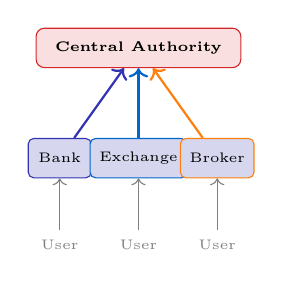
\begin{tikzpicture}
      % Central authority at top
      \node[draw=mlred, fill=mlred!15, rounded corners=3pt,
            font=\tiny\bfseries, align=center, minimum width=2.6cm, minimum height=0.5cm]
            (ca) at (0,3.2) {Central Authority};
      % Three pillars below
      \node[draw=mlpurple, fill=mllavender4, rounded corners=2pt,
            font=\tiny, align=center, minimum width=0.8cm, minimum height=0.5cm]
            (bank) at (-1.0,1.8) {Bank};
      \node[draw=mlblue, fill=mllavender4, rounded corners=2pt,
            font=\tiny, align=center, minimum width=0.8cm, minimum height=0.5cm]
            (exch) at (0,1.8) {Exchange};
      \node[draw=mlorange, fill=mllavender4, rounded corners=2pt,
            font=\tiny, align=center, minimum width=0.8cm, minimum height=0.5cm]
            (brok) at (1.0,1.8) {Broker};
      % Arrows up to central authority
      \draw[->, mlpurple, thick] (bank) -- (ca);
      \draw[->, mlblue, thick]   (exch) -- (ca);
      \draw[->, mlorange, thick] (brok) -- (ca);
      % Users at bottom
      \node[font=\tiny, mlgray, align=center] (u1) at (-1.0,0.7) {User};
      \node[font=\tiny, mlgray, align=center] (u2) at (0,0.7) {User};
      \node[font=\tiny, mlgray, align=center] (u3) at (1.0,0.7) {User};
      \draw[->, mlgray] (u1) -- (bank);
      \draw[->, mlgray] (u2) -- (exch);
      \draw[->, mlgray] (u3) -- (brok);
    \end{tikzpicture}
  \end{column}

  \begin{column}{0.24\textwidth}
    \centering
    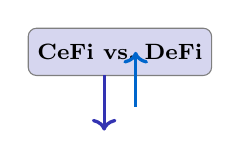
\begin{tikzpicture}
      \node[draw=mlgray, fill=mllavender4, rounded corners=3pt,
            font=\footnotesize\bfseries, align=center,
            minimum width=2.0cm, minimum height=0.6cm]
            at (0,1.5) {CeFi vs.\ DeFi};
      \draw[->, very thick, mlpurple] (-0.2,1.2) -- (-0.2,0.5);
      \draw[->, very thick, mlblue]   ( 0.2,0.8) -- ( 0.2,1.5);
    \end{tikzpicture}
  \end{column}

  \begin{column}{0.38\textwidth}
    \centering
    {\small\bfseries\color{mlgreen} Decentralised Finance (DeFi)}\\[0.3cm]
    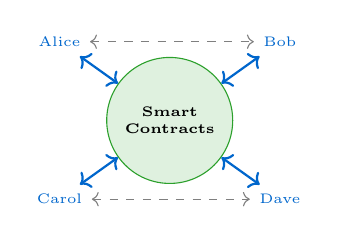
\begin{tikzpicture}
      % Smart contracts centre
      \node[draw=mlgreen, fill=mlgreen!15, circle,
            font=\tiny\bfseries, align=center,
            minimum width=1.6cm] (sc) at (0,2.0) {Smart\\Contracts};
      % Users around it
      \node[font=\tiny, mlblue, align=center] (ua) at (-1.4,3.0) {Alice};
      \node[font=\tiny, mlblue, align=center] (ub) at ( 1.4,3.0) {Bob};
      \node[font=\tiny, mlblue, align=center] (uc) at (-1.4,1.0) {Carol};
      \node[font=\tiny, mlblue, align=center] (ud) at ( 1.4,1.0) {Dave};
      \draw[<->, mlblue, thick] (ua) -- (sc);
      \draw[<->, mlblue, thick] (ub) -- (sc);
      \draw[<->, mlblue, thick] (uc) -- (sc);
      \draw[<->, mlblue, thick] (ud) -- (sc);
      % Peer arrows
      \draw[<->, mlgray, dashed] (ua) -- (ub);
      \draw[<->, mlgray, dashed] (uc) -- (ud);
    \end{tikzpicture}
  \end{column}
\end{columns}

\vspace{0.2cm}
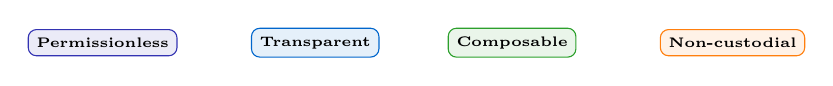
\begin{tikzpicture}
  \node[draw=mlpurple,  fill=mlpurple!10,  rounded corners=3pt, font=\tiny\bfseries, inner sep=3pt] at (1.5,0) {Permissionless};
  \node[draw=mlblue,    fill=mlblue!10,    rounded corners=3pt, font=\tiny\bfseries, inner sep=3pt] at (4.2,0) {Transparent};
  \node[draw=mlgreen,   fill=mlgreen!10,   rounded corners=3pt, font=\tiny\bfseries, inner sep=3pt] at (6.7,0) {Composable};
  \node[draw=mlorange,  fill=mlorange!10,  rounded corners=3pt, font=\tiny\bfseries, inner sep=3pt] at (9.5,0) {Non-custodial};
\end{tikzpicture}

\bottomnote{DeFi = financial services built on public blockchains, governed by smart contracts.}
\end{frame}

% ==================== FRAME 4: THE DeFi STACK ====================
\begin{frame}{The DeFi Stack}
\centering
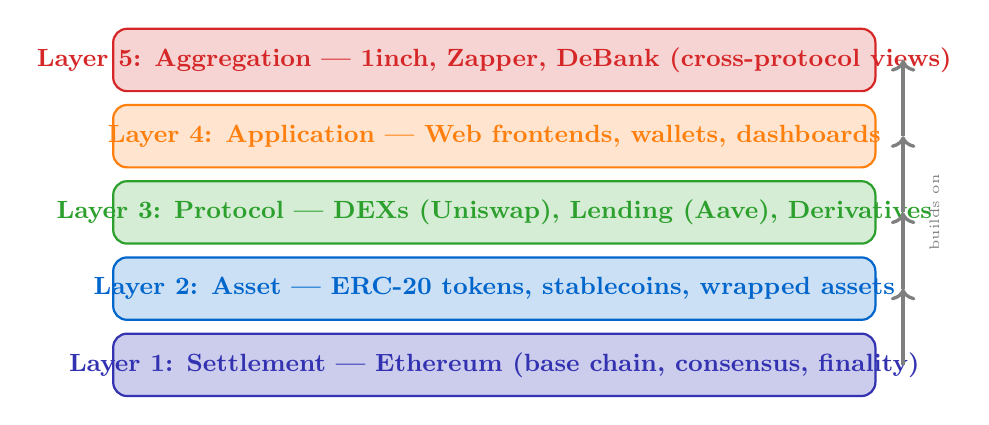
\begin{tikzpicture}[scale=0.88]
  % Layer 1 -- Settlement
  \draw[fill=mlpurple!25, draw=mlpurple, rounded corners=5pt, thick]
       (0,0) rectangle (11,0.9);
  \node[font=\small\bfseries, mlpurple, align=center] at (5.5,0.45)
       {Layer 1: Settlement --- Ethereum (base chain, consensus, finality)};

  % Layer 2 -- Asset
  \draw[fill=mlblue!20, draw=mlblue, rounded corners=5pt, thick]
       (0,1.1) rectangle (11,2.0);
  \node[font=\small\bfseries, mlblue, align=center] at (5.5,1.55)
       {Layer 2: Asset --- ERC-20 tokens, stablecoins, wrapped assets};

  % Layer 3 -- Protocol
  \draw[fill=mlgreen!20, draw=mlgreen, rounded corners=5pt, thick]
       (0,2.2) rectangle (11,3.1);
  \node[font=\small\bfseries, mlgreen, align=center] at (5.5,2.65)
       {Layer 3: Protocol --- DEXs (Uniswap), Lending (Aave), Derivatives};

  % Layer 4 -- Application
  \draw[fill=mlorange!20, draw=mlorange, rounded corners=5pt, thick]
       (0,3.3) rectangle (11,4.2);
  \node[font=\small\bfseries, mlorange, align=center] at (5.5,3.75)
       {Layer 4: Application --- Web frontends, wallets, dashboards};

  % Layer 5 -- Aggregation
  \draw[fill=mlred!20, draw=mlred, rounded corners=5pt, thick]
       (0,4.4) rectangle (11,5.3);
  \node[font=\small\bfseries, mlred, align=center] at (5.5,4.85)
       {Layer 5: Aggregation --- 1inch, Zapper, DeBank (cross-protocol views)};

  % Upward arrows between layers
  \draw[->, very thick, mlgray] (11.4,0.45) -- (11.4,1.55);
  \draw[->, very thick, mlgray] (11.4,1.55) -- (11.4,2.65);
  \draw[->, very thick, mlgray] (11.4,2.65) -- (11.4,3.75);
  \draw[->, very thick, mlgray] (11.4,3.75) -- (11.4,4.85);
  \node[font=\tiny, mlgray, rotate=90] at (11.85,2.65) {builds on};
\end{tikzpicture}

\bottomnote{DeFi is built in composable layers -- each layer builds on those below it.}
\end{frame}

% ==================== FRAME 5: HOW DEXs WORK ====================
\begin{frame}{How DEXs Work}

\begin{tikzpicture}[remember picture, overlay]
  % Panel borders
  \draw[thick, mlpurple, rounded corners=3pt] (0.1,0.2) rectangle (4.0,4.2);
  \draw[thick, mlblue,   rounded corners=3pt] (4.3,0.2) rectangle (8.2,4.2);
  \draw[thick, mlgreen,  rounded corners=3pt] (8.5,0.2) rectangle (12.4,4.2);

  % --- Panel 1: CEX order book ---
  \node[font=\tiny\bfseries, mlpurple] at (2.05,3.9) {CEX Order Book};
  % Bid column
  \draw[fill=mlgreen!20, mlgreen] (0.3,2.8) rectangle (1.7,3.6);
  \node[font=\tiny, mlgreen, align=center] at (1.0,3.2) {BID\\100 @ 1800\\200 @ 1795};
  % Ask column
  \draw[fill=mlred!20, mlred] (2.2,2.8) rectangle (3.6,3.6);
  \node[font=\tiny, mlred, align=center] at (2.9,3.2) {ASK\\50 @ 1805\\150 @ 1810};
  % Matchmaker
  \draw[fill=mlpurple!15, mlpurple, rounded corners=2pt] (1.2,1.7) rectangle (2.8,2.5);
  \node[font=\tiny\bfseries, mlpurple, align=center] at (2.0,2.1) {Match\\maker};
  \draw[->, mlpurple] (1.4,2.8) -- (1.6,2.5);
  \draw[->, mlpurple] (2.6,2.8) -- (2.4,2.5);
  % Users
  \node[font=\tiny, mlgray] at (0.7,1.1) {Buyer};
  \node[font=\tiny, mlgray] at (3.3,1.1) {Seller};
  \draw[->, mlgray] (0.7,1.3) -- (1.5,1.7);
  \draw[->, mlgray] (3.3,1.3) -- (2.5,1.7);
  \node[font=\tiny\bfseries, mlpurple] at (2.05,0.45) {Panel 1};

  % --- Panel 2: Alice wanting to swap ---
  \node[font=\tiny\bfseries, mlblue] at (6.25,3.9) {Alice wants to swap};
  % Alice stick figure
  \draw[mlblue,thick] (5.3,2.8) circle (0.18);
  \draw[mlblue,thick] (5.3,2.62) -- (5.3,2.15);
  \draw[mlblue,thick] (5.3,2.45) -- (5.0,2.25);
  \draw[mlblue,thick] (5.3,2.45) -- (5.6,2.25);
  \draw[mlblue,thick] (5.3,2.15) -- (5.05,1.85);
  \draw[mlblue,thick] (5.3,2.15) -- (5.55,1.85);
  % ETH -> USDC arrow
  \node[font=\tiny\bfseries, mlpurple] at (6.0,2.7) {ETH};
  \draw[->, very thick, mlblue] (6.3,2.7) -- (7.0,2.7);
  \node[font=\tiny\bfseries, mlgreen] at (7.3,2.7) {USDC};
  % Question bubble
  \draw[fill=white, mlblue, rounded corners=2pt] (4.5,1.2) rectangle (8.0,1.9);
  \node[font=\tiny, mlblue, align=center] at (6.25,1.55) {But who holds my funds?\\No custodian needed!};
  \node[font=\tiny\bfseries, mlblue] at (6.25,0.45) {Panel 2};

  % --- Panel 3: AMM pool ---
  \node[font=\tiny\bfseries, mlgreen] at (10.45,3.9) {AMM Pool};
  % Pool container
  \draw[fill=mlblue!15, draw=mlblue, thick, rounded corners=4pt]
       (8.7,2.0) rectangle (10.1,3.6);
  \node[font=\tiny\bfseries, mlblue, align=center] at (9.4,2.8) {ETH\\Pool};
  \draw[fill=mlgreen!15, draw=mlgreen, thick, rounded corners=4pt]
       (10.3,2.0) rectangle (11.7,3.6);
  \node[font=\tiny\bfseries, mlgreen, align=center] at (11.0,2.8) {USDC\\Pool};
  % Swap arrow
  \draw[<->, very thick, mlorange] (9.4,1.8) -- (9.4,1.2) -- (11.0,1.2) -- (11.0,1.8);
  \node[font=\tiny, mlorange] at (10.2,1.05) {swap};
  % x*y=k badge
  \draw[fill=mlpurple, rounded corners=3pt] (9.3,0.5) rectangle (11.5,0.95);
  \node[font=\small\bfseries, white] at (10.4,0.72) {$x \cdot y = k$};
  \node[font=\tiny\bfseries, mlgreen] at (10.45,0.20) {Panel 3};
\end{tikzpicture}

\bottomnote{DEXs replace order books with liquidity pools governed by a constant-product formula.}
\end{frame}

% ==================== FRAME 6: LIQUIDITY POOLS ====================
\begin{frame}{Liquidity Pools Visualised}
\centering
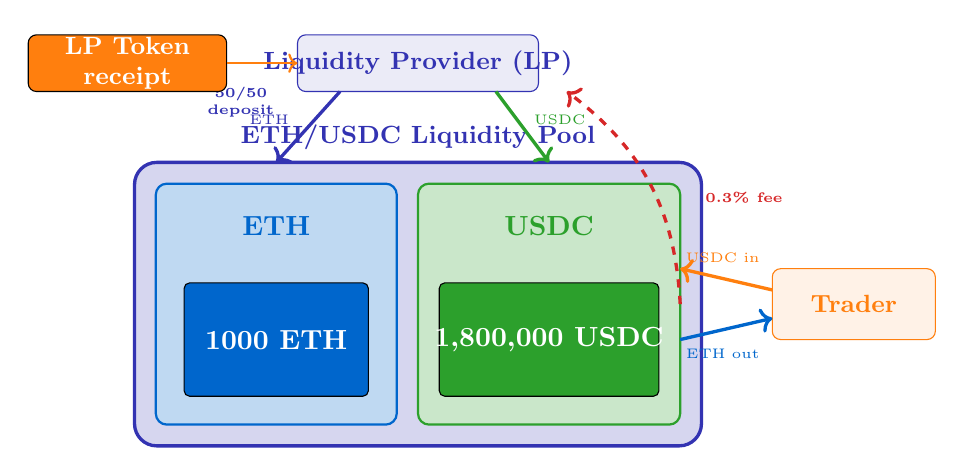
\begin{tikzpicture}[scale=0.9]
  % Main pool container
  \draw[fill=mllavender4, draw=mlpurple, very thick, rounded corners=8pt]
       (1.5,0.5) rectangle (9.5,4.5);
  \node[font=\bfseries\small, mlpurple] at (5.5,4.85) {ETH/USDC Liquidity Pool};

  % ETH compartment (left half)
  \draw[fill=mlblue!25, draw=mlblue, thick, rounded corners=4pt]
       (1.8,0.8) rectangle (5.2,4.2);
  \node[font=\bfseries, mlblue] at (3.5,3.6) {ETH};
  \draw[fill=mlblue, rounded corners=2pt] (2.2,1.2) rectangle (4.8,2.8);
  \node[font=\normalsize\bfseries, white] at (3.5,2.0) {1000 ETH};

  % USDC compartment (right half)
  \draw[fill=mlgreen!25, draw=mlgreen, thick, rounded corners=4pt]
       (5.5,0.8) rectangle (9.2,4.2);
  \node[font=\bfseries, mlgreen] at (7.35,3.6) {USDC};
  \draw[fill=mlgreen, rounded corners=2pt] (5.8,1.2) rectangle (8.9,2.8);
  \node[font=\normalsize\bfseries, white] at (7.35,2.0) {1,800,000 USDC};

  % LP depositing from top
  \draw[fill=mlpurple!10, draw=mlpurple, rounded corners=3pt]
       (3.8,5.5) rectangle (7.2,6.3);
  \node[font=\small\bfseries, mlpurple, align=center] at (5.5,5.9)
       {Liquidity Provider (LP)};
  \draw[->, very thick, mlpurple] (4.4,5.5) -- (3.5,4.5);
  \draw[->, very thick, mlgreen]  (6.6,5.5) -- (7.35,4.5);
  \node[font=\tiny, mlpurple] at (3.4,5.1) {ETH};
  \node[font=\tiny, mlgreen]   at (7.5,5.1) {USDC};
  \node[font=\tiny\bfseries, mlpurple, align=center] at (3.0,5.35) {50/50\\deposit};

  % Trader swapping from right side
  \draw[fill=mlorange!10, draw=mlorange, rounded corners=3pt]
       (10.5,2.0) rectangle (12.8,3.0);
  \node[font=\small\bfseries, mlorange, align=center] at (11.65,2.5) {Trader};
  \draw[->, very thick, mlorange] (10.5,2.7) -- (9.2,3.0);
  \draw[<-, very thick, mlblue]   (10.5,2.3) -- (9.2,2.0);
  \node[font=\tiny, mlorange] at (9.8,3.15) {USDC in};
  \node[font=\tiny, mlblue]   at (9.8,1.8)  {ETH out};

  % Fee arrows back to LP
  \draw[->, very thick, mlred, dashed] (9.2,2.5) to[bend right=25] (7.6,5.5);
  \node[font=\tiny\bfseries, mlred] at (10.1,4.0) {0.3\% fee};

  % LP Token badge
  \draw[fill=mlorange, rounded corners=3pt] (0.0,5.5) rectangle (2.8,6.3);
  \node[font=\small\bfseries, white, align=center] at (1.4,5.9) {LP Token\\receipt};
  \draw[->, thick, mlorange] (2.8,5.9) -- (3.8,5.9);
\end{tikzpicture}

\bottomnote{Liquidity providers deposit equal value of two tokens and earn trading fees.}
\end{frame}

% ==================== FRAME 7: LENDING AND BORROWING ====================
\begin{frame}{DeFi Lending and Borrowing}
\begin{columns}[c]
  \begin{column}{0.38\textwidth}
    \centering
    {\small\bfseries\color{mlblue} Lender}\\[0.2cm]
    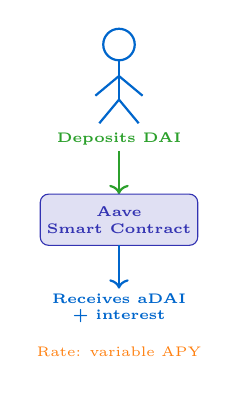
\begin{tikzpicture}
      % Lender figure
      \draw[mlblue,thick] (1.5,4.2) circle (0.2);
      \draw[mlblue,thick] (1.5,4.0) -- (1.5,3.5);
      \draw[mlblue,thick] (1.5,3.8) -- (1.2,3.55);
      \draw[mlblue,thick] (1.5,3.8) -- (1.8,3.55);
      \draw[mlblue,thick] (1.5,3.5) -- (1.25,3.2);
      \draw[mlblue,thick] (1.5,3.5) -- (1.75,3.2);
      % Deposit DAI arrow
      \node[font=\tiny\bfseries, mlgreen] at (1.5,3.0) {Deposits DAI};
      \draw[->, thick, mlgreen] (1.5,2.85) -- (1.5,2.3);
      % Aave protocol box
      \draw[fill=mlpurple!15, draw=mlpurple, rounded corners=3pt,
            minimum width=2.0cm, minimum height=0.6cm]
           (0.5,1.65) rectangle (2.5,2.3);
      \node[font=\tiny\bfseries, mlpurple, align=center] at (1.5,1.97) {Aave\\Smart Contract};
      % Receives aDAI arrow
      \draw[->, thick, mlblue] (1.5,1.65) -- (1.5,1.1);
      \node[font=\tiny\bfseries, mlblue, align=center] at (1.5,0.85) {Receives aDAI\\+ interest};
      % Interest rate
      \node[font=\tiny, mlorange] at (1.5,0.3) {Rate: variable APY};
    \end{tikzpicture}
  \end{column}

  \begin{column}{0.24\textwidth}
    \centering
    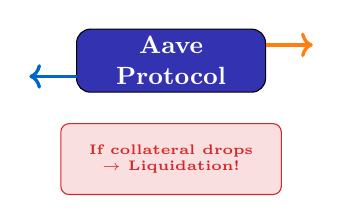
\begin{tikzpicture}
      \draw[fill=mlpurple, rounded corners=5pt] (-0.2,1.3) rectangle (2.2,2.1);
      \node[font=\small\bfseries, white, align=center] at (1.0,1.7) {Aave\\Protocol};
      \draw[->, very thick, mlblue]  (-0.2,1.5) -- (-0.8,1.5);
      \draw[->, very thick, mlorange] (2.2,1.9) -- (2.8,1.9);
      % Warning box at bottom
      \draw[fill=mlred!15, draw=mlred, rounded corners=3pt]
           (-0.4,0.0) rectangle (2.4,0.9);
      \node[font=\tiny\bfseries, mlred, align=center] at (1.0,0.45)
           {If collateral drops\\$\rightarrow$ Liquidation!};
    \end{tikzpicture}
  \end{column}

  \begin{column}{0.38\textwidth}
    \centering
    {\small\bfseries\color{mlorange} Borrower}\\[0.2cm]
    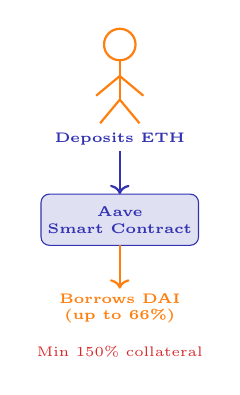
\begin{tikzpicture}
      % Borrower figure
      \draw[mlorange,thick] (1.5,4.2) circle (0.2);
      \draw[mlorange,thick] (1.5,4.0) -- (1.5,3.5);
      \draw[mlorange,thick] (1.5,3.8) -- (1.2,3.55);
      \draw[mlorange,thick] (1.5,3.8) -- (1.8,3.55);
      \draw[mlorange,thick] (1.5,3.5) -- (1.25,3.2);
      \draw[mlorange,thick] (1.5,3.5) -- (1.75,3.2);
      % Deposit ETH collateral arrow
      \node[font=\tiny\bfseries, mlpurple] at (1.5,3.0) {Deposits ETH};
      \draw[->, thick, mlpurple] (1.5,2.85) -- (1.5,2.3);
      % Aave protocol box
      \draw[fill=mlpurple!15, draw=mlpurple, rounded corners=3pt,
            minimum width=2.0cm, minimum height=0.6cm]
           (0.5,1.65) rectangle (2.5,2.3);
      \node[font=\tiny\bfseries, mlpurple, align=center] at (1.5,1.97) {Aave\\Smart Contract};
      % Borrows DAI arrow
      \draw[->, thick, mlorange] (1.5,1.65) -- (1.5,1.1);
      \node[font=\tiny\bfseries, mlorange, align=center] at (1.5,0.85) {Borrows DAI\\(up to 66\%)};
      % Collateral ratio
      \node[font=\tiny, mlred] at (1.5,0.3) {Min 150\% collateral};
    \end{tikzpicture}
  \end{column}
\end{columns}

\bottomnote{DeFi lending is overcollateralized -- borrowers must deposit more than they borrow.}
\end{frame}

% ==================== FRAME 8: DeFi BY THE NUMBERS ====================
\begin{frame}{DeFi by the Numbers}
\centering
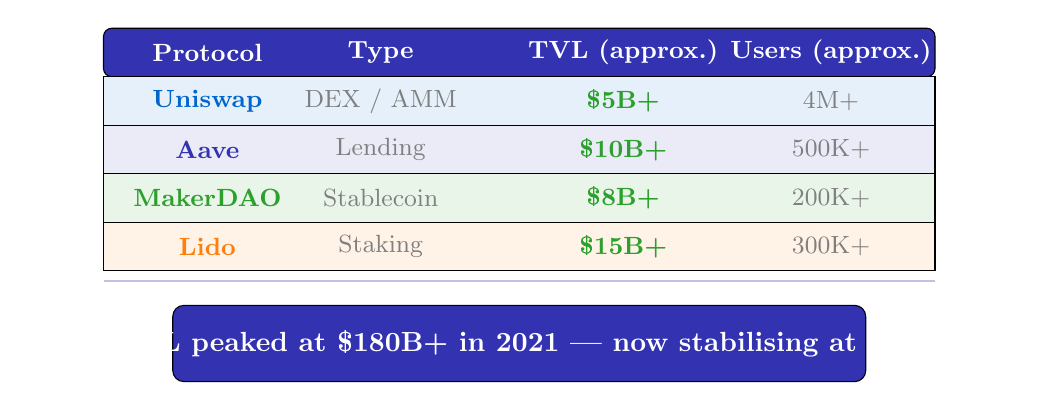
\begin{tikzpicture}[scale=0.88]
  % Table header
  \draw[fill=mlpurple, rounded corners=3pt] (0,5.2) rectangle (12,5.9);
  \node[font=\small\bfseries, white] at (1.5,5.55) {Protocol};
  \node[font=\small\bfseries, white] at (4.0,5.55) {Type};
  \node[font=\small\bfseries, white] at (7.5,5.55) {TVL (approx.)};
  \node[font=\small\bfseries, white] at (10.5,5.55) {Users (approx.)};

  % Row 1 -- Uniswap
  \draw[fill=mlblue!10] (0,4.5) rectangle (12,5.2);
  \node[font=\small\bfseries, mlblue] at (1.5,4.85) {Uniswap};
  \node[font=\small, mlgray, align=center] at (4.0,4.85) {DEX / AMM};
  \node[font=\small\bfseries, mlgreen] at (7.5,4.85) {\$5B+};
  \node[font=\small, mlgray] at (10.5,4.85) {4M+};

  % Row 2 -- Aave
  \draw[fill=mlpurple!10] (0,3.8) rectangle (12,4.5);
  \node[font=\small\bfseries, mlpurple] at (1.5,4.15) {Aave};
  \node[font=\small, mlgray] at (4.0,4.15) {Lending};
  \node[font=\small\bfseries, mlgreen] at (7.5,4.15) {\$10B+};
  \node[font=\small, mlgray] at (10.5,4.15) {500K+};

  % Row 3 -- MakerDAO
  \draw[fill=mlgreen!10] (0,3.1) rectangle (12,3.8);
  \node[font=\small\bfseries, mlgreen] at (1.5,3.45) {MakerDAO};
  \node[font=\small, mlgray] at (4.0,3.45) {Stablecoin};
  \node[font=\small\bfseries, mlgreen] at (7.5,3.45) {\$8B+};
  \node[font=\small, mlgray] at (10.5,3.45) {200K+};

  % Row 4 -- Lido
  \draw[fill=mlorange!10] (0,2.4) rectangle (12,3.1);
  \node[font=\small\bfseries, mlorange] at (1.5,2.75) {Lido};
  \node[font=\small, mlgray] at (4.0,2.75) {Staking};
  \node[font=\small\bfseries, mlgreen] at (7.5,2.75) {\$15B+};
  \node[font=\small, mlgray] at (10.5,2.75) {300K+};

  % Divider
  \draw[mllavender2, thick] (0,2.25) -- (12,2.25);

  % Summary bar
  \draw[fill=mlpurple, rounded corners=4pt] (1.0,0.8) rectangle (11.0,1.9);
  \node[font=\normalsize\bfseries, white, align=center] at (6.0,1.35)
       {DeFi TVL peaked at \$180B+ in 2021 --- now stabilising at \$50--100B};
\end{tikzpicture}

\bottomnote{TVL (Total Value Locked) measures total assets deposited in DeFi protocols.}
\end{frame}

% ==================== FRAME 9: THE RISKS ====================
\begin{frame}{The Risks of DeFi}

\begin{tikzpicture}[remember picture, overlay]
  % Panel borders
  \draw[thick, mlgreen,  rounded corners=3pt] (0.1,0.2) rectangle (4.0,4.2);
  \draw[thick, mlred,    rounded corners=3pt] (4.3,0.2) rectangle (8.2,4.2);
  \draw[thick, mlpurple, rounded corners=3pt] (8.5,0.2) rectangle (12.4,4.2);

  % --- Panel 1: Happy developer ---
  \node[font=\tiny\bfseries, mlgreen] at (2.05,3.9) {Deploying\ldots};
  % Developer stick figure (happy)
  \draw[mlgreen,thick] (2.05,3.3) circle (0.22);
  % Smile
  \draw[mlgreen,thick] (1.92,3.22) arc (210:330:0.13);
  \draw[mlgreen,thick] (2.05,3.08) -- (2.05,2.55);
  \draw[mlgreen,thick] (2.05,2.85) -- (1.7,2.6);
  \draw[mlgreen,thick] (2.05,2.85) -- (2.4,2.6);
  \draw[mlgreen,thick] (2.05,2.55) -- (1.75,2.2);
  \draw[mlgreen,thick] (2.05,2.55) -- (2.35,2.2);
  % Laptop
  \draw[fill=mllavender4, draw=mlpurple]    (0.5,0.8) rectangle (3.6,1.8);
  \draw[fill=mllavender3, draw=mlpurple]    (0.7,1.0) rectangle (3.4,1.7);
  \node[font=\tiny\bfseries, mlgreen] at (2.05,1.35) {Contract deployed!};
  % Speech bubble
  \draw[fill=white, mlgreen, rounded corners=2pt] (0.4,2.0) rectangle (3.7,2.4);
  \node[font=\tiny, mlgreen, align=center] at (2.05,2.2) {My smart contract is live!};
  \node[font=\tiny\bfseries, mlgreen] at (2.05,0.45) {Panel 1};

  % --- Panel 2: Hacker exploiting ---
  \node[font=\tiny\bfseries, mlred] at (6.25,3.9) {Exploit!};
  % Hacker figure (masked)
  \draw[mlred,thick] (5.6,3.3) circle (0.22);
  \draw[fill=mlred!30, mlred] (5.38,3.3) rectangle (5.82,3.52);
  \node[font=\tiny, mlred] at (5.6,3.41) {mask};
  \draw[mlred,thick] (5.6,3.08) -- (5.6,2.55);
  \draw[mlred,thick] (5.6,2.85) -- (5.3,2.6);
  \draw[mlred,thick] (5.6,2.85) -- (5.9,2.6);
  \draw[mlred,thick] (5.6,2.55) -- (5.3,2.2);
  \draw[mlred,thick] (5.6,2.55) -- (5.9,2.2);
  % Attack arrows with labels
  \draw[->, thick, mlred] (6.3,3.1) -- (7.8,3.5);
  \node[font=\tiny, mlred, align=left] at (7.2,3.7) {Reentrancy};
  \draw[->, thick, mlorange] (6.3,2.7) -- (7.8,2.5);
  \node[font=\tiny, mlorange, align=left] at (7.2,2.35) {Oracle\\manipulation};
  \draw[->, thick, mlpurple] (6.3,2.2) -- (7.8,1.8);
  \node[font=\tiny, mlpurple, align=left] at (7.15,1.65) {Flash loan\\attack};
  % Funds stolen
  \node[font=\small\bfseries, mlred] at (6.25,1.0) {\$\$\$ drained!};
  \node[font=\tiny\bfseries, mlred] at (6.25,0.45) {Panel 2};

  % --- Panel 3: Solutions shield ---
  \node[font=\tiny\bfseries, mlpurple] at (10.45,3.9) {Defence};
  % Shield shape
  \draw[fill=mlpurple!15, draw=mlpurple, very thick]
       (9.2,1.0) -- (9.2,3.3) -- (10.45,3.7) -- (11.7,3.3) -- (11.7,1.0) -- (10.45,0.5) -- cycle;
  % Solutions inside shield
  \node[font=\tiny\bfseries, mlpurple, align=center] at (10.45,3.1) {Formal\\Verification};
  \node[font=\tiny\bfseries, mlblue, align=center]   at (10.45,2.5) {Smart Contract\\Audits};
  \node[font=\tiny\bfseries, mlgreen, align=center]  at (10.45,1.9) {Bug Bounties};
  \node[font=\tiny\bfseries, mlorange, align=center] at (10.45,1.35) {On-chain\\Insurance};
  \node[font=\tiny\bfseries, mlpurple] at (10.45,0.45) {Panel 3};
\end{tikzpicture}

\bottomnote{Smart contract bugs are permanent -- DeFi protocols need audits, insurance, and formal verification.}
\end{frame}

% ==================== FRAME 10: KEY TAKEAWAYS ====================
\begin{frame}{Key Takeaways}
\centering
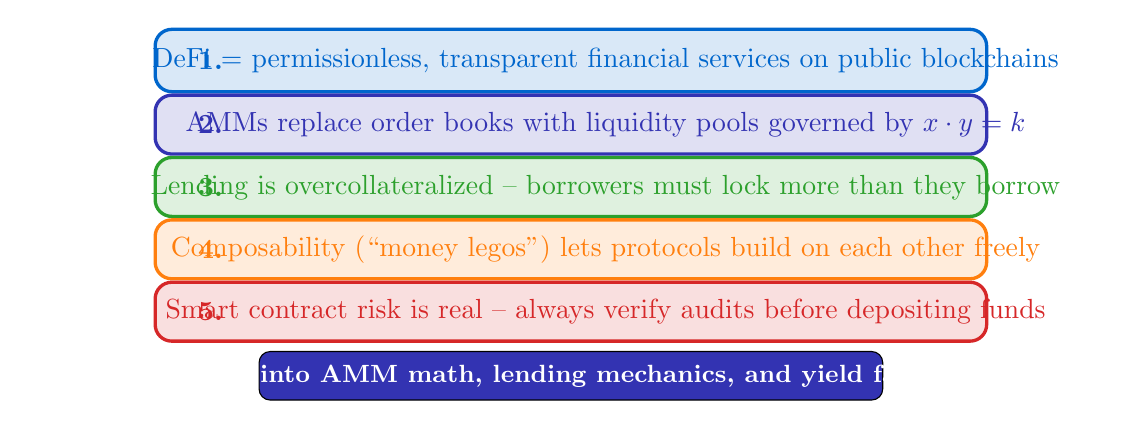
\begin{tikzpicture}[scale=0.88]
  % Box 1
  \draw[fill=mlblue!15, draw=mlblue, very thick, rounded corners=6pt]
       (0,4.5) rectangle (12,5.4);
  \node[font=\normalsize\bfseries, mlblue] at (0.8,4.95) {1.};
  \node[font=\normalsize, mlblue, align=left] at (6.5,4.95)
       {DeFi = permissionless, transparent financial services on public blockchains};

  % Box 2
  \draw[fill=mlpurple!15, draw=mlpurple, very thick, rounded corners=6pt]
       (0,3.6) rectangle (12,4.45);
  \node[font=\normalsize\bfseries, mlpurple] at (0.8,4.02) {2.};
  \node[font=\normalsize, mlpurple, align=left] at (6.5,4.02)
       {AMMs replace order books with liquidity pools governed by $x \cdot y = k$};

  % Box 3
  \draw[fill=mlgreen!15, draw=mlgreen, very thick, rounded corners=6pt]
       (0,2.7) rectangle (12,3.55);
  \node[font=\normalsize\bfseries, mlgreen] at (0.8,3.12) {3.};
  \node[font=\normalsize, mlgreen, align=left] at (6.5,3.12)
       {Lending is overcollateralized -- borrowers must lock more than they borrow};

  % Box 4
  \draw[fill=mlorange!15, draw=mlorange, very thick, rounded corners=6pt]
       (0,1.8) rectangle (12,2.65);
  \node[font=\normalsize\bfseries, mlorange] at (0.8,2.22) {4.};
  \node[font=\normalsize, mlorange, align=left] at (6.5,2.22)
       {Composability (``money legos'') lets protocols build on each other freely};

  % Box 5
  \draw[fill=mlred!15, draw=mlred, very thick, rounded corners=6pt]
       (0,0.9) rectangle (12,1.75);
  \node[font=\normalsize\bfseries, mlred] at (0.8,1.32) {5.};
  \node[font=\normalsize, mlred, align=left] at (6.5,1.32)
       {Smart contract risk is real -- always verify audits before depositing funds};

  % Teaser
  \draw[fill=mlpurple, rounded corners=4pt] (1.5,0.05) rectangle (10.5,0.75);
  \node[font=\small\bfseries, white, align=center] at (6.0,0.40)
       {Next: Deep dive into AMM math, lending mechanics, and yield farming strategies};
\end{tikzpicture}

\bottomnote{Next: Deep dive into AMM math, lending mechanics, and yield farming strategies.}
\end{frame}

\end{document}
